\documentclass{article}
\usepackage{graphicx} % Required for inserting images
\usepackage{cite}
\usepackage{setspace}
\usepackage{verbatimbox}

\title{NHL Meter}
\author{Alexander Hagood \& Alexander Barran}
\date{November 2024}
\doublespacing
\begin{document}

\maketitle

\section{Abstract}
The objective of this project is to provide a system that can provide live estimates of the outcomes of a National Hockey League (NHL) game.
Using statistical and machine learning methods, we were able to create a model applying logistic regression. This model can sucessfully forecast
the outcome of live NHL games with a high degree of accuracy.

\section{Introduction}
Inspired by visualizations such as the Win Probability graph provided by ESPN, we sought to create a similar metric based on hockey play-by-play data sourced from the NHL.
We would like to use information about the state of the game, such as the current score, 'momentum,' and other factors that can be derived from the data to determine the odds of the home team winning at any arbitrary point in the game.
Sports are inherently unpredictable; however, we can still make educated guesses at the chances of specific outcomes based on information we have.
Our approach is to stream 'Play-by-Play' data representing certain game events into our model, and then use statistical and machine learning techniques such as logistic regression and machine learning to update our estimation of who is more likely to win as we gain more information about the state of the game.


\section{Problem Definition}
Given the Play-By-Play data for a specific NHL match up to a certain time point, 
what is the probability of the Home or Away team winning? With the rise of the sports
betting industry, these types of endeavor have grown in popularity and interest on
both the bettor and bookkeeper sides, as bettors seek new edges and bookkeepers seek
to set more accurate lines. Estimates of NHL outcomes are not new, but from our research,
there is no investigation into the dynamic estimation as the game is played. Measuring
this probability can give us insight into the nature the moment an underdog team might
turn the tables on a strong team, or show how a dominant team can maintain control of the game.

\section{Models, Algorithms and Measures}
\subsection{Why Logistic Regression?}
While this project largely represents a binary classification problem in picking between one of two teams as the victor, we chose to use a logistic regression rather than a typical classification algorithm.
This is because the goal is not to predict the winning team, but to give the odds for a team to win based on the current game state.
Classification models like K-Nearest Neighbors would not have given us the flexibility to use confidence intervals as a form of win probability.
We then picked the logistic regression since we assume that the factors affecting a win are not linear.
The \texttt{LogisticRegression} class from \texttt{scikit-learn} provides a function called \texttt{predict\_proba()} which will return the model's confidence that a sample belongs to class 0 or class 1.
In our case, class 0 represents a home win and class 1 represents an away win.

\subsection{Determining Team Strength with Elo}
In order to measure the comparative strength of two teams, it is not necessary to reinvent the wheel. 
Elo is a metric that lets us quantify this strength in a of teams, derived from the results of previous head-to-head match ups.
Upon completing a game, you receive Elo score corresponding to the difference between your score and your opponents. Win a game against
an opponent with a much higher score, and you receive more points than winning one with a lower score, and vice versa for losing.
Once you have these scores, you can measure the probability of a given team winning against another in a match up. 
Using the following formula we can determine the probability of a given Elo matchup resulting in a win.
\[E_{A} = \frac{1}{1 + 10^{(R_{B} - R_{A})/400}}\] 

\section{Implementation and Analysis}
\subsection{Data Retrieval, Cleaning, and Explanation}
Our data is sourced from the official NHL API.
This allows you to get historical play-by-play data from games since the 2007 season using HTTP requests in JSON format.
The library \texttt{hockey-scraper} by harryshomer on PyPI allows you to input a season or a date range, and will download the season information then all associated plays with each game in that season.
This is a large amount of data, representing nearly 700,000 plays between the 2007-2008 and 2023-2024 seasons.
Due to API rate limiting, this download took multiple days.
The data was placed into Pandas DataFrame objects and saved to parquet files.
Post-parquet compression, the data for play-by-play and shifts (documenting when a player comes on or off the ice) took up approximately half a gigabyte.

Analyzing the format of the data, we can view useful information about the game.
A "play" is recorded whenever a notable event occurs.
These events can take many forms such as a shot on goal, a successful goal, the result of a face-off, penalties, or other associated game events. 
Every play lists all players that were involved, as well as all other players on the ice at the time.
Spatial data is included, such as the X and Y coordinates on the rink where the event happened.
Each play also lists information about the game state such as the current score, the teams, and the time remaining in the period.

\subsection{Regression Features}
In order to start adjusting the probability of a given team winning, you need a beginning assumption.
One could just assume that each team has an equal chance of winning, but this naive assumption neglects the individuality of teams and players.
We chose to use the Elo system to determine this assumption.
Starting in the 2007 season, we gave each team a base level of 1500 Elo, and then started feeding in the results of their match ups.
Roster and staff changes for teams between seasons make it unreasonable to assume that their Elo will be the same between seasons.
To maintain some continuity, we shift every team's back Elo by one-third of their difference to the baseline rather than completely resetting to 1500.
One special case in this system was the Atlanta Thrashers, who relocated to Winnipeg in 2011 to become the Winnipeg Jets.
Since the team also moved their players and staff to the new location, the "new" Winnipeg Jets inherited the Atlanta Thrashers' Elo.
We can now feed in this Elo score to get a baseline win probability when analyzing specific games.

We can start to adjust winning probability based on game events by first using each team's Elo score entering the game.
Then, we divide the game into discrete time slices of 30 seconds.
Each time slice represents the game state at the end of each interval, including each team's total score, shots on goal, hits, strength, and penalty minutes.
Power plays are an important event for two to five minutes that can increase scoring chances and change the outcome of the game, and must be properly accounted for by the model.
The original NHL dataset represents the number of players on the ice as strings like "5x5" or "4x5", where the first number shows the home team's strength and the second shows the away team's strength.
Since these strings cannot be fed into the logistic regression model, the strengths are converted into the home team's player differential.
Thus, "5x5" or "even strength" becomes 0, and "4x5" becomes -1, and vice versa.

In the NHL, games will advance to overtime if the score is tied at the end of three periods.
For the regular season, teams play one, five-minute overtime of 3-on-3 before going to a shootout.
For the playoffs, this is increased to unlimited twenty minute periods of 5-on-5 until one team scores.
Due to this unpredictability and the puzzle for handling time remaining when the game length is unknown, we decided to remove overtime games from the dataset.
Now that the time remaining feature ranges from 3600 (three, twenty minute periods, in seconds) to zero, we normalized the time remaining between 0 and 1 by dividing by 3600.

\subsection{Model Training and Validation}
The \texttt{LogisticRegression} model uses the \texttt{liblinear} solver for binary classification and \texttt{l2} penalty regularization.
To select the best penalty, we trained multiple models using different penalties ranging from 0.00001 to 1.0.
The accuracy of each model was compared using repeated K-fold cross validation with 10 splits and 3 repeats.
The Matplotlib chart in Figure \ref{fig:kfold} shows each model's accuracy.
We moved forward with the 1.0 penalty for having the best mean accuracy and smallest quartile range.

It is important to discuss the meaning of this accuracy statistic and why it is not necessarily a good measure of our final product.
For any given play, the model has approximately a 79\% chance of predicting the correct winner.
The following testing section will discuss better strategies in detail.

\begin{figure}
    \centering
    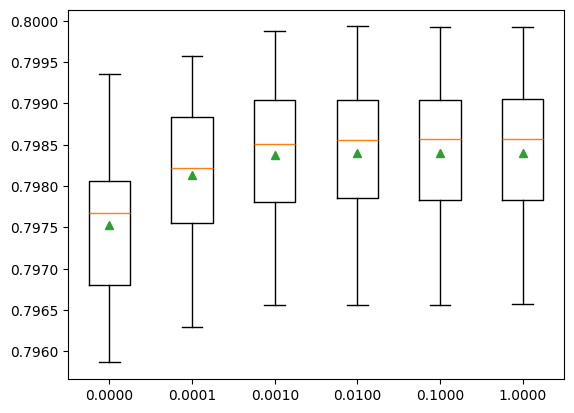
\includegraphics[width=0.75\linewidth]{kfold.png}
    \caption{Repeated Stratified K-Fold Cross Validation on Logistic Regression}
    \label{fig:kfold}
\end{figure}

\subsection{Testing}
There is clearly no objective answer representing the true probability of a team winning given a given set of circumstances that we can compare our results to.
However, we can measure how accurately our model can predict probabilities in aggregate by 'backtesting' it.
There are two different methodologies we came up with to backtest our model. 

The first type we came up with is through using statistical regression methods. 
First, we group together games or plays with similar expected outcomes, such as all games around 70\% home team win probability. We can then see measure how often
the home team won in this set of games, and compare it to our model's prediction. We repeat this for all probability 'buckets' which can be at any arbitrary precision.
Once we have the True win rate, and the expected win rate, we can perform statistical methods to such as sum of least squares or logistic loss. These functions measure 'Goodness of Fit,' 
or generally represent how accurate our model is. 

There exist other types of backtesting that we can apply that are called 'scoring rules.' These are evaluation metrics that can be used to evaluate the accuracy of probabilistic predictions.
These types of scoring rules are highly applicable to our project, as we are directly making these types of forecasts and would like to measure their accuracy. By using these rules we can attempt to minimize our distance from true probability.
The scoring function we used is called Ranked Probability Score. Using the backtesting functions on the Elo model, we can see the following results:


  \begin{verbatim}
    Sum of Least Squares: 12.2505
    Cross Entropy: 0.8863
    Ranked Probability Score: 0.1228
  \end{verbatim}

We now can confirm that Elo is an acceptable model for predicting the outcomes on a game level, as the closer the RPS is to 0 the better.


\section{Results and Discussion}
The trained model can now approach the game state time series data to plot a team's win probability over time.
Three types of games will be the most interesting to analyze: comebacks, blowouts, and late go-ahead goals.

In the 2010 NHL Playoffs, the Philadelphia Flyers were once down 0-3 in their series against the Boston Bruins.
The Flyers rallied to force a Game 7, but fell to a score of 0-3 during the first period.
Over the next forty-five minutes, the Flyers put up four goals against the Bruins to advance to the Eastern Conference Final.

\begin{figure}
    \centering
    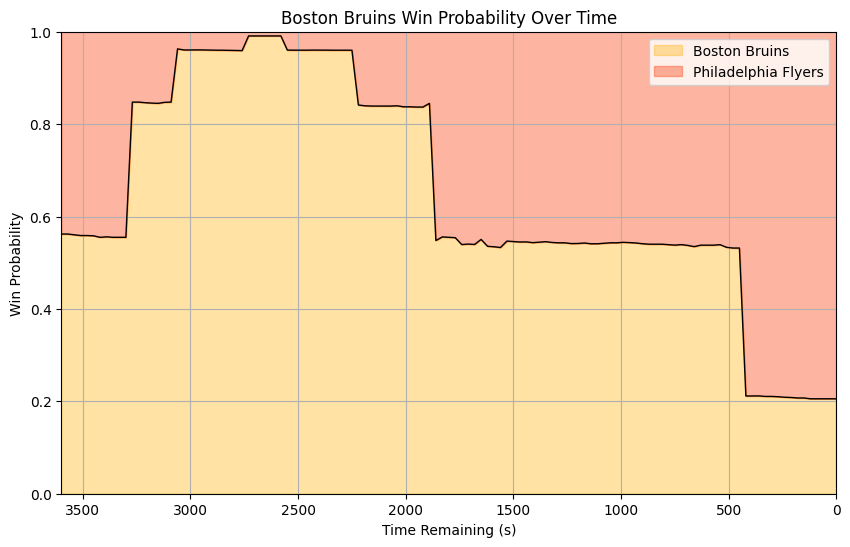
\includegraphics[width=1.0\linewidth]{2009030227.png}
    \caption{Philadelphia Flyers at Boston Bruins, 14 May 2010}
    \label{fig:comeback}
\end{figure}

The game events are clearly represented in Figure \ref{fig:comeback}.
Entering the game with the higher Elo, the Boston Bruins started with a marginally higher win probability than their opponent.
Being the defining factor in winning and losing, goals have the most impact on the win probability.
Each significant jump shows a goal, such as the Bruins' first goal of the night 5:27 into the first period.
Their early work in the game showed their win probability approach 100\%, being up three goals with higher momentum.
A Flyers' goal late in the first period made little impact as they still lagged in score, hits, and shots on goal.

A notable event type affecting the probabilities throughout are power plays.
Less than one minute after the Flyers' game-tying third goal, they received a two minute minor penalty for high-sticking.
During this time, they played at a one player disadvantage.
For these two minutes, Boston's win probability elevated.
One minute following Philadelphia's successful penalty kill, the Bruins were indicted for hooking.
For these two minutes, their win probability drops slightly.

On April 7, 2009, the Carolina Hurricanes recorded the biggest shutout of the 21st century.
Shown in Figure \ref{fig:shutout}, Carolina starts with a strong 72\% win probability as they enter as strong favorites with an Elo 193 points higher than New York.
Beginning with Dennis Seidenberg's slap shot goal 2:54 into the first period, the Hurricanes would go on to score nine goals to the Islanders zero.
With no response to the Carolina onslaught, the Y-axis for win probability had to be shifted to start at 0.7 and never dropped below the starting mark.
Successive goals push the Hurricanes' win probability to an irrecoverable 99.9\% before the halfway point of the game.

\begin{figure}
    \centering
    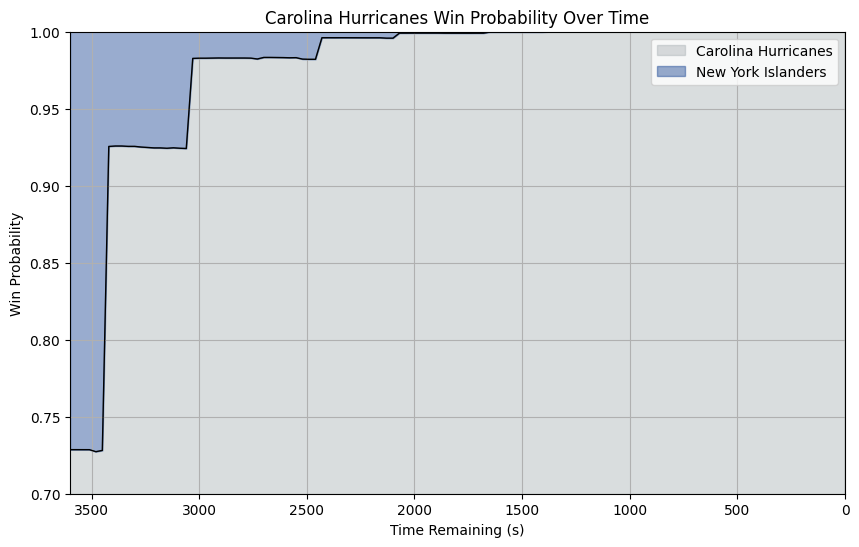
\includegraphics[width=1.0\linewidth]{2008021187.png}
    \caption{New York Islanders at Carolina Hurricanes, 7 April 2009}
    \label{fig:shutout}
\end{figure}

On January 24, 2021, the Edmonton Oilers and Winnipeg Jets were tied at 3 goals each near the end of the third period.
Figure \ref{fig:goahead} shows just the win probability over just the third period, which Edmonton entered leading 2-1.
Two goals in less than two minutes by the Jets turned the tides in their favor, until the Oilers tied it again with four minutes to go.
An overtime period was set to cap off an exciting night where both teams led by one goal for long stretches.
With less than one second remaining in regulation, Leon Draisaitl of the Oilers scored to put Edmonton up 4-3 over Winnipeg.
The graph shows this sudden lead change and effect of the last-second goal on the game's outcome.

\begin{figure}
    \centering
    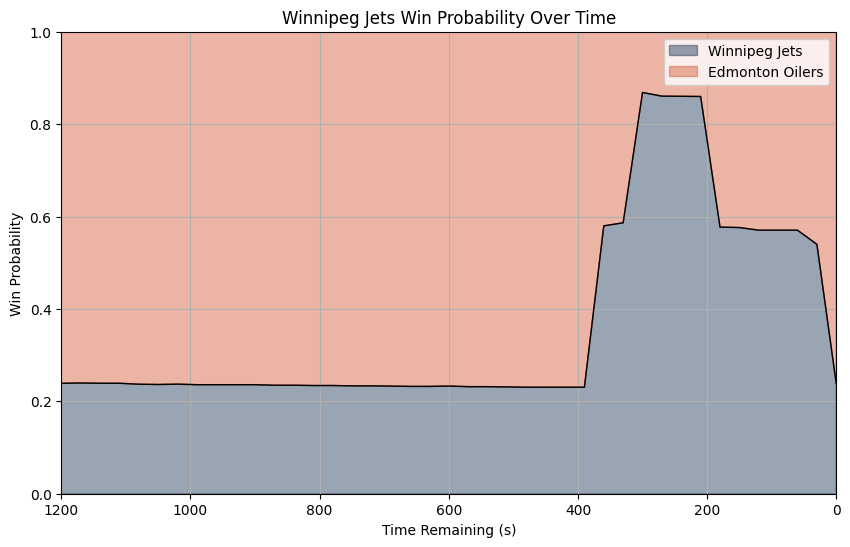
\includegraphics[width=1\linewidth]{2020020086.png}
    \caption{Edmonton Oilers at Winnipeg Jets, 24 January 2021}
    \label{fig:goahead}
\end{figure}

Analyzing our model with our backtesting functions, we the following numerical results


\begin{verbatim}
Sum of Least Squares: 0.0525
Cross Entropy: 0.4951
Ranked Probability Score: 0.0668
\end{verbatim}

These results show a strong ability to predict the outcome of a game given the game state, and that our model is accurate. For example, for RPS a score closer to 0 is better, so our model is twice as accurate
at predicting the outcomes of games as the Elo model. This indicates our model is closely following the true probability of NHL games.

\subsection{Discussion}
One weakness of this model is its apparent inability to adjust the win probability as the time remaining approaches zero.
Looking back at Figure \ref{fig:comeback}, the win probability for the Bruins with no time remaining should be zero considering they are down one goal with no opportunity to score.
However, their chance hovers near 20\% for the game duration after the Flyers' final goal.
Similarly in Figure \ref{fig:goahead}, the Jets' win probability against a last-second go-ahead goal hovers near 20\%.

We also find that man advantages are not properly accounted for.
The model weights goals so heavily that significant scoring opportunities like power plays have a negligible impact on the win probability.
Teams with strong power play units can convert a power play into a goal between 20\% and 30\% of the time \cite{powerplay}.
However, since our feature set abstracts a team into an Elo score, the model is oblivious to a team's power play strengths or weaknesses.
Including a team's power play percentage is beyond the scope of this project, and we predict that it may introduce correlation with Elo.
One scenario that the features also ignore is a team pulling their goalie.
Usually performed by a trailing team late in the game, this allows a team to put six skaters on the ice for additional offensive pressure.
It comes at the cost of an empty net, and greatly increases the opposing team's scoring chances \cite{goaliepull}.
Since the strength feature will only represent this as a 1 or -1, it is treated the same as a power play which typically has the opposite effect on win probability.

\section{Related Work}
Similar work in this field has been done for other sports, such as the aforementioned ESPN Win Probability graph.
Some of the most useful work in this field has been done by groups studying Soccer like American Soccer Analysis using a 
machine learning based approach \cite{richardett} or research by Robberechts et al \cite{bayesian} using Bayesian methods. Soccer
is a much more translatable sport to our problem, as it is also a low scoring game with a similar gameplay flow to hockey.
These works served as useful inspiration and insight into how we could develop an approach to predict the outcomes of hockey games.

\section{Conclusion}
In this project, we have developed a model that can predict the outcomes of NHL games based on the game state. Using our logistic regression model, we were able to display the estimated probability of 
a team winning at any given point in the game. We have shown that our model is accurate at predicting the outcomes of games using statistical methods such as sum of least squares and ranked probability score,
showing our model is twice as accurate as using just Elo. Improvements to this model in the future may be the ability to adapt the program to stream in data live, and extending the model to be able to interpret games that 
go into overtime.

\nocite{*}
\bibliographystyle{IEEEtran}
\bibliography{references}
\end{document}